%%%%%%%%%%%%%%%%%%%%%%%%%%%%%%% TO DOS %%%%%%%%%%%%%%%%%%%%%%%%%%%%%%%
% 1. 
%%%%%%%%%%%%%%%%%%%%%%%%%%%%%%%%%%%%%%%%%%%%%%%%%%%%%%%%%%%%%%%%%%%%%%

\section{Introduction} 
\label{sec:intro}
%%%%%%%%%%%%%%%%%%%%%%%%%%%%%%%%% DCC is here %%%%%%%%%%%%%%%%%%%%%%%%%%%%%%%%%%
Today's datacenters (DCs) are server-centric: users rent servers with
specific hardware capabilities tailored to their needs (e.g.,
compute-intensive EC2 instances from Amazon). 
A \emph{disaggregated} datacenter (DDC) disaggregates, or separates,
the resources in a traditional DC into resource \emph{blades},
with each resource connected directly to an interconnect (Figure~\ref{fig:DDC}). 
We use the term \emph{blade} to describe a 1U server containing one resource
type, and \emph{resource} for an individual CPU, DIMM, SSD, etc. in a blade. 

%%%%%%%%%%%%%%%%%%%%%%%%%%%%%%%%% DDC benefits %%%%%%%%%%%%%%%%%%%%%%%%%%%%%%%%%

The modularity of DDCs benefits both operators and
users~\cite{Han2013}. By separating resources into blades, a
DDC provides efficiency: the operator can upgrade specific hardware
blades without impacting other resources types. Users also experience
an efficiency win: in a DDC a user can provision the exact amount of
resources they require and dynamically expand/shrink this set. This flexibility
also increases the DC resource utilization.

%%%%%%%%%%%%%%%%%%%%%%%%%%%%% Research challenges %%%%%%%%%%%%%%%%%%%%%%%%%%%%%%

% Recent research has shown that DDCs are now
% practical~\cite{IntelRSA,Gao2016,Lim2009,Lim2012}. Most research has focused
% on building DDCs~\cite{IntelRSA}, network requirements~\cite{Gao2016}, or
% memory and storage disaggregation solutions~\cite{Lim2009,Lim2012}. 
% \todo{Add decibel and Facebook disaggregated rack}. 

% \ac{Seems out of place.} Gao et al. explored the network requirements for DDCs
% and found that the network
% needs to have at most 3--5$\mu$s latency and at least 40Gbps of 
% \emph{application} bandwidth~\cite{Gao2016}.  However, because the
% disaggregation of servers into blades is a fundamental change to the DC
% architecture, the resource management is an open research question.

There are two broad types of disaggregation: partial and full.
In partial disaggregation compute resources have a small amount of
local memory, %% to act as a cache
memory and storage resources have CPUs, % to manage accesses,
and a NIC is attached to each resource. 
In full disaggregation each resource is independent and is directly
connected to the rack interconnect. Current research focuses on the practicality
of partial disaggregation~\cite{IntelRSA,Gao2016,Lim2009,Lim2012}.

In this paper, we discuss partial disaggregation at rack-scale:
% Rack-scale disaggregation is where disaggregation occurs within the rack.
resources can only connect to other resources in the same rack (e.g., a CPU in
rack1 cannot connect to a DIMM in rack2).
% and can only directly connect to a
%resource within its own rack.
The disaggregated rack is presented to the
client as a single machine through a virtualization layer. Applications can
request a number of VMs to allocate among the racks.
Distributed applications might then run among several disaggregated racks, while
a single-machine application will reside in one rack. %\ac{choppy} What happens
% if one resource fails in a rack?

%\ac{Need a transition.}

%%%%%%%%%%%%%%%%%%%%%%%%%%%%%%%%%%%%%%%%%%%%%%%%%%%%%%%%%%%%%%%%%%%%%%%%%%%%%%%%
\begin{figure}
    \centering
    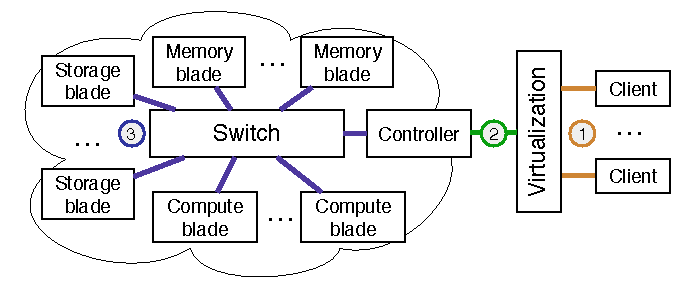
\includegraphics[width=\columnwidth]{fig/ddc-overview}
    \caption{Simplified representation of a disaggregated datacenter with
    three communication points: (1) between the application and the
    virtualization layer,
    (2) between the virtualization layer and the physical resources, and (3)
    between the physical resources bundled as blades.}
    \label{fig:DDC}
\end{figure}
%%%%%%%%%%%%%%%%%%%%%%%%%%%%%%%%%%%%%%%%%%%%%%%%%%%%%%%%%%%%%%%%%%%%%%%%%%%%%%%%

%%%%%%%%%%%%%%%%%%%%%%%%%%%%%%%% We focus on FT %%%%%%%%%%%%%%%%%%%%%%%%%%%%%%%%

% In this paper we explore this question by looking at the fault tolerance of
% resource blades in a DDC. As a starting point we only consider crash failures as
% these are the easiest to reason about. 

%% , when a resource halts, but worked correctly before halting

% Fine-grained failures can occur in a DDC because  

Disaggregation requires a re-thinking of failure assumptions core to
existing application designs. We expect that DDC designs will make it
possible for resource failures to no longer fate-share: a failure of a
memory resource will not cause the failure of the CPU that was using
that memory resource. In a traditional DC, complex applications take
on the responsibility of dealing with server failures. But, such
legacy applications are not disaggregation-aware, and should not be
expected to handle individual resource failures in a DDC. So, how
should the CPU respond when it cannot write to a memory resource? And,
more importantly, should a developer deploying their code in a DDS be
expected to reason about and account for failures of individual
resources?

% \ac{Mihir noted that this should state it is inefficient to run legacy
% applications on a DDC without any fault tolerance. The applications can still
% run, but will not be able to take advantage of the modularity.}
% Applications written for traditional server-centric datacenters cannot account
% for individual resource failures. 
For example, distributed data processing platforms like Hadoop, Naiad,
and Spark use system-specific fault tolerance schemes to recover from
server failures. However, %% These applications are expected to be resilient to
%% failure, but
they cannot recover from resource
failures~\cite{Dean2004,Murray2013,Zaharia2012}. In the case of resource
failure, the entire application would fail, leading these applications to
run inefficiently on Dec's. It's not unreasonable
to expect legacy DC application to run in DDCs without modification but still
take advantage of DDC modularity.
%% between a DC and DDC, therefore resource failures must be explicitly
%% handled.
Since such legacy, disaggregation-unaware, applications cannot efficiently handle
resource failures, DDCs must provide infrastructure and system support
for coping with such failures.

%% as it would require them to reason
%% about disaggregation. The cluster scheduler would need to determine if
%% computation must be redone or if it simply needs to reroute
%% communication. This is not realistic to require of applications.

% Therefore,
% resource failures must be presented to the application as failures it can reason
% about.

%\ac{Need transition.}

%%%%%%%%%%%%%%%%%%%%%%%%%%%%%%%%% We propose... %%%%%%%%%%%%%%%%%%%%%%%%%%%%%%%%

In this paper we explore the co-design of DDC fault tolerance with the network by expanding the
role of software defined networking (SDN). An SDN controller has
a global view of the network and can dynamically reconfigure routing~\cite{Feamster2014,Jarschel2014,Sezer2013}. Both
features are useful in managing DDC resources. A controller and the
switch can be implemented such that the controller is notified of new
resources, the health of each resource, etc. Therefore, the controller
can collect information about each resource in its rack. The
dynamic flow rule changes will allow the network to react to events,
such as failures or resource additions. The above is not difficult to achieve as
many DCs already use SDN-capable ToR switches.

% At first glance moving resource failure recovery into the network appears to be
% contrary to the end-to-end principle~\cite{Saltzer1984}. We are not, however,
% proposing to remove application-level failure handling entirely; instead, we
% propose to improve performance by reducing the number of failure cases that the
% application level must handle. For example, we do not handle arbitrary or
% byzantine failures, these must be handled by the application.

%% \ac{This needs work to be integrated better. I'm having a hard time finding a
%% good place for it in the introduction.}

%%%%%%%%%%%% Key choice of FT in DDC is granularity of fate sharing %%%%%%%%%%%%

We believe that one key choice in designing fault tolerance for DDCs is the
\emph{granularity of resource fate sharing}. Since DDCs present an environment where
no fate sharing exists, what should be exposed to the application?
Should the failures be visible or transparent? And, if they are visible,
should they be presented as a server failure? 
%
We believe that network-driven failure recovery in DDCs can be used to
present legacy application with types of failure that can appear in
a traditional DC (e.g., server failure).
%
We break down possible fault tolerance designs based on the
granularity of fate sharing (Figure~\ref{fig:spectrum}): VM-level
(complete fate sharing), process-level (partial fate sharing), and no
fate sharing. We believe that these three granularities, covered in
more detail in Section~\ref{sec:design}, are sufficient for most
legacy applications.

Some applications, particularly those designed for a disaggregated
environment may benefit from a fate sharing granularity that is
different from the three types above. %% They might benefit
%% from other fate sharing granularities not present in traditional
%% datacenters.
A file system that prioritizes strong consistency over
availability may want to fate share a CPU resource that serializes
operations with all but one disk resource. This system would retain
strong consistency guarantees even if the serializing mechanism fails
by retaining a single (serializing) disk resource, and failing the
other disk resources.
%
%% We will give several examples to motivate the need for more flexible
%% fate sharing arrangements.
%
%% We show there is not one fate sharing model which allows
%% all application types to benefit from DDC modularity.
Considering a broad diversity of fate sharing models, how can DDCs
provide fault tolerance? We argue that fate sharing granularity and failure mitigation should
be \emph{programmable}, allowing applications to choose the most
appropriate fate sharing arrangement. 

There are two places where this programmability can be implemented:
the application and the (software defined) network. We argue that the
network is the right place for this programmability. First, failure
detection and mitigation can be more easily and more efficiently
implemented by the network, especially in a DDC where all
inter-resource communication is observable by the network. Second, the
network is a natural place to enforce DDC resource fate sharing.
%
Moving programmability into the network appears to be contrary to the
end-to-end principle~\cite{Saltzer1984}. We are not, however,
proposing to remove application-level failure handling entirely; for
example, our proposed mechanisms will not handle a broad range of
faults such as byzantine failures (these must still be handled by the
application). But we do argue that, in line with the end-to-end
principle, certain resource faults can be more efficiently dealt with
by the network.

% \todo{Discuss non-legacy applications and programmability.}

%
%% The network must also detect the failure before the application can to
%% avoid any side effects from the application observing the failure.
%
% We also discuss other requirements to replicate expected application
%% network driven failure recovery must maintain the same
% failure semantics. 



% Complete fate sharing causes any resource failure
% to cause a VM instance failure. Partial fate sharing leaves the fate sharing
% enforcement for CPU blades up to the application and recovers from memory blade
% failures. No fate sharing recovers both CPU and memory blade failures for the
% application.

%%%%%%%%%%%%%%%%%%%%%%%%%%%%%%%%% Why network? %%%%%%%%%%%%%%%%%%%%%%%%%%%%%%%%%
% The failure recovery of resource blades should be in line with
% the benefits and goals of disaggregation, but the fault tolerance design cannot
% make assumptions about the applications running in the datacenter.

% To allow legacy applications to work in DDCs, applications cannot be
% disaggregation-aware, which requires the datacenter to handle the
% individual resource failures for the application. Providing
% applications with transparent fault tolerance has been done before at
% the virtual machine or hypervisor
% level~\cite{Bressoud1995,Cully2008,Lorch2015}. However, these
% solutions are inappropriate for low-latency environments. For example,
% Remus~\cite{Cully2008} utilizes speculative execution to keep
% replicated VMs in near lock step and requires all output to be
% buffered for an epoch. Once the epoch is reached, the system is
% checkpointed and the output is flushed. DDCs require low latency due
% to the disaggregated nature of the resources. Therefore, Remus-style
% solutions, where the tail-latencies are dependent on the epoch, are
% inappropriate for DDCs.

%% \ac{Need to introduce ``traditional'' and ``non-traditional'' fate sharing
%% models earlier.}

%%%%%%%%%%%%%%%%%%%%%%%%%%%%%%%% Contributions %%%%%%%%%%%%%%%%%%%%%%%%%%%%%%%%%

In summary, we describe existing DC fate sharing models ported to DDCs using
SDN in the context of several sample applications. We then describe requirements for new
fate sharing models made possible by DDCs and the applications that can benefit
from these. Through our analysis, we noticed that different classes of
applications require different fate sharing semantics. Some
applications can benefit from previously unattainable fate sharing
models with small changes. To achieve the full benefit of disaggregation for
both legacy applications and new applications, we argue that fate sharing must
be both \emph{programmable} and \emph{solved by the network}. We sketch out
a design for how this might be achieved and discuss outstanding challenges.
